%%%%%%%%%%%%%%%%%%%%%%%%
%
% $Author: Achal Shakywar $
% $Datum: 15.12.2023  $
% $Pfad: MLProject\ML23-01-Keyword-Spotting-with-an-Arduino-Nano-33-BLE-Sense\report\Images\Domain\ModelTrainingFlow.tex$
% $Version: 1.0 $
%
% !TeX encoding = utf8
%
%%%%%%%%%%%%%%%%%%%%%%%%

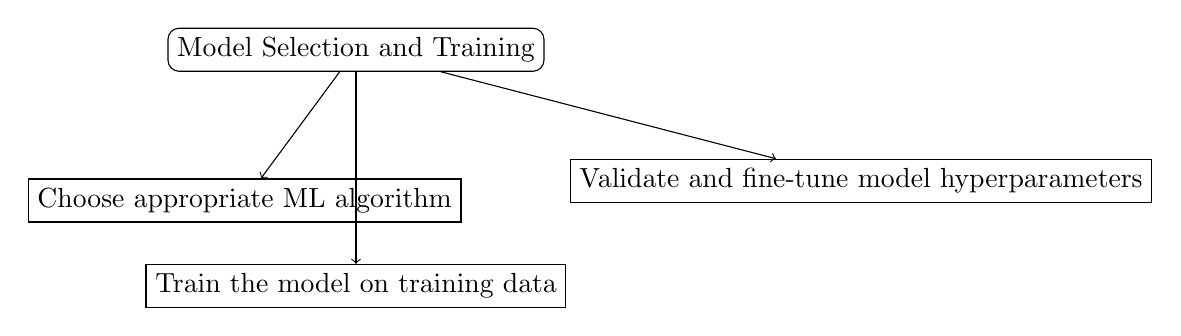
\begin{tikzpicture}[node distance=2cm, auto]
	% Nodes
	\node (model) [draw, rounded corners] {Model Selection and Training};
	\node (algo) [draw, below left of=model, xshift=-0cm, yshift=-0.5cm] {Choose appropriate ML algorithm};
	\node (train) [draw, below of=model, yshift=-1cm] {Train the model on training data};
	\node (validate) [draw, below right of=model, xshift=5cm, yshift=-0.25cm] {Validate and fine-tune model hyperparameters};
	
	% Arrows
	\draw [->] (model) -- (algo);
	\draw [->] (model) -- (train);
	\draw [->] (model) -- (validate);
	
\end{tikzpicture}
